\section{Introduction}
\label{sec:evolution-introduction}

\subsection{Tree representation of Keyword-driven Tests}
\label{sec:tree-representation-KDT}

KDT tests can be represented using a tree structure. Figure~\ref{fig:robotframework_tree} shows this structure for the test of Figure~\ref{fig:robot-script}. The root of the tree (purple rectangle) is the \emph{Test Case} that is executed by calling all the keywords contained. The intermediary nodes (white rectangles) are called \emph{User Keywords} since they are created by the tester. Finally, the leaf nodes (green rectangles) are \emph{Library Keywords}. \emph{Library Keywords} are implemented by the system or an external library and responsible for either controlling the control flow of the tests or interacting with the SUT.

\begin{figure}
\centering
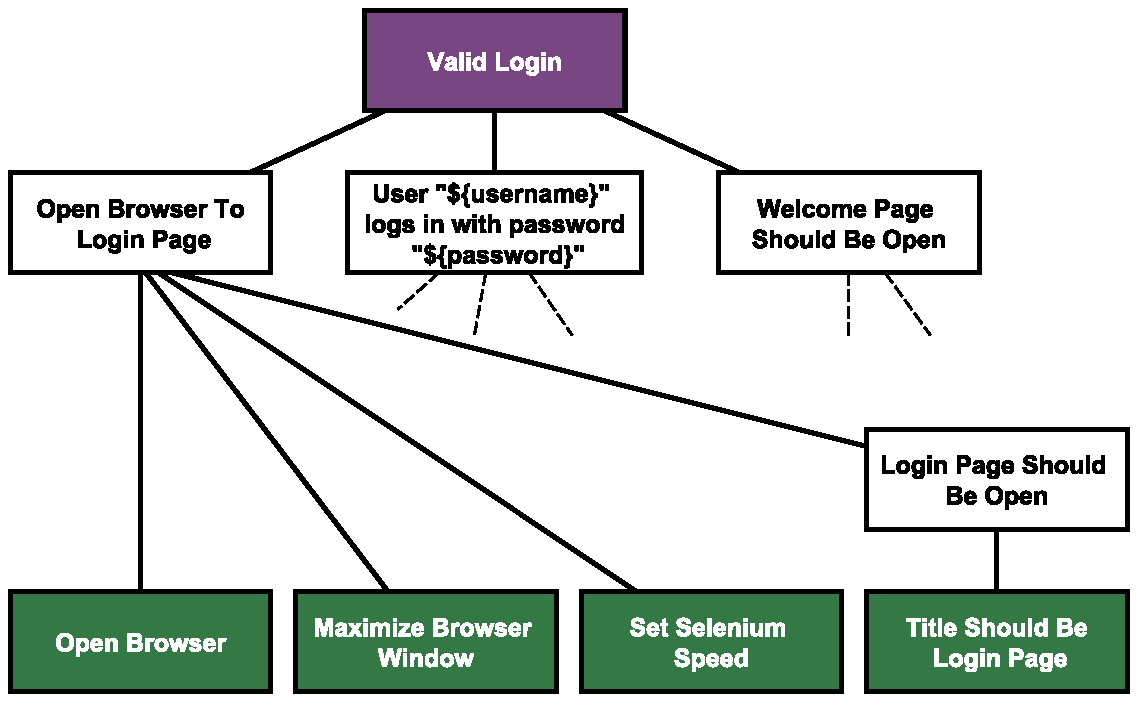
\includegraphics[width=0.7\columnwidth]{figures/evolution/robotframework_tree.pdf}
\caption{Tree representation of the ``Valid Login'' KDT test.}
\label{fig:robotframework_tree}
\end{figure}

We group keywords into seven categories based on their functionality and present them in Table \ref{keywords_categories}. We define a \emph{SYNC} keyword category for keywords dealing with the synchronization between tests and SUT; e.g., a keyword that waits 10 seconds for a GUI element of the SUT to become available. In the rest of the paper we use the term keyword to refer to \emph{User Keywords} unless stated otherwise.

\begin{table}
\caption{Keyword categories}
\label{keywords_categories}
\centering
\begin{tabular}{>{\raggedright}m{0.9in}>{\raggedright}m{4in}}
\toprule
\textbf{\scriptsize{Label}} & \textbf{\scriptsize{Explanation}}\tabularnewline
\toprule

\scriptsize{\textit{ACTION}} & \scriptsize{Keyword performing an action on the
SUT capable of modifying its state.} \tabularnewline

\scriptsize{\textit{ASSERTION}} & \scriptsize{Keyword verifying that a predicate
is true at a specific point of test execution} \tabularnewline

\scriptsize{CONTROLFOW} & \scriptsize{Keyword allowing to modify the
                                   control flow of the test execution.} \tabularnewline

\scriptsize{GETTER} & \scriptsize{Keyword allowing to extract an element from
the SUT.} \tabularnewline

\scriptsize{LOGGING} & \scriptsize{Keyword dumping logs during execution.}
\tabularnewline

\scriptsize{SYNC} & \scriptsize{Keyword relating to the
                                  synchronization between the SUT and the tests.} \tabularnewline

\scriptsize{\textit{USER}} & \scriptsize{Keyword created by a user.}
\tabularnewline

\bottomrule
\end{tabular}
\end{table}


One the tools used for the application of KDT is Robot Framework \cite{RobotFramework2020}. Robot Framework is a popular framework used world-wide by major companies, including Nokia, KONE, ABB. This is also the tool adopted by our industrial partner and, thus, used in this work. Robot Framework is an open source tool originally developed by Nokia Networks and is mainly used for acceptance testing. The ``Valid Login'' KDT test of Figure~\ref{fig:robot-script} was written using this framework.

One of the main advantages of Robot Framework is its high modularity.  Indeed, Robot Framework is platform-agnostic and thanks to its driver plugin architecture, the core framework does not require any knowledge of the SUT. For instance, in Figure~\ref{fig:robot-script}, lines 1--2 show that the script is using the external library for Selenium to interact with the SUT. Another advantage of the framework lies in its simple syntax, which makes it easily accessible to testers, regardless of their background.

\subsection{Industrial Context}
\label{sec:evolution-introduction-data}

In this work, we aim at investigating the evolution of KDT test suites at the acceptance testing level based on the industrial practice. To this end, we work together with BGL BNP Paribas that has recently (1 year ago) adopted KDT and uses it in its daily software development work for acceptance testing.

One of the reasons that our partner adopted KDT is that test cases at this testing level were created by different domain experts (business analysts and automation experts) and the adoption of a common language between the experts was imperative. All the tests used in our study have been created by a team of 3 testers and 2 business analysts working at BGL BNP Paribas using Robot Framework.

The project used in our study, hereafter referred to as \emph{SubjectA} for confidentiality reasons, pertains to all the business activities of our partner. The front-end is a web application implemented in AngularJS, and, the back-end is composed of hundreds of services written in various programming languages. These services are managed by different teams, involving more than 100 developers. The KDT test suite used in our study, referred to as \emph{TestSuiteA}, is developed by 3 testers working at the Quality Assurance (QA) team of our partner and 2 business analysts.

\begin{figure}[t!]
  \centering
  \includegraphics[width=0.7\columnwidth]{figures/evolution/project_evolution.pdf}
  \caption{Evolution of TestSuiteA}
  \label{fig:project_evolution}%\setlength{\tabcolsep}{5.1px} 
\end{figure}

Figure~\ref{fig:project_evolution} shows the evolution of TestSuiteA across the eight-month period studied. The figure depicts the evolution of the number of \emph{Test Cases} comprising the test suite, the number of \emph{User Keywords} and the lines of code of the test suite. As can be seen, our analysis begins with a test suite of 39 test cases, 139 user keywords and 1129 lines of code and ends with 117 test cases, 505 keywords and 4732 lines of code.

In the time span depicted in Figure~\ref{fig:project_evolution}, we isolated three periods during which we saw an increased test creation activity (shown in grey). After discussing with the QA team, they corroborated that these periods were more focused on test creation and the remaining ones on test maintenance. Thus, we analyze separately these periods (greyed and non-greyed) and refer to them as ``Creation'' and ``Maintenance''.